\section{Graph of Evolutionary Transitions}
\paragraph{}
In section \ref{sec:themeExtraction} we showed a method to extract themes from the dataset of articles over a given period of time. However we are interested in detecting events that can last for a long time. This is why we studied evolutionary transitions. In section \ref{sec:EvoGraphInterest} we introduce the Kullback-Leibler divergence which allows to measure the distance between extracted themes and we show how it can be interpreted to detect long lasting events. Then, in section \ref{sec:EvoGraphImplementation} and \ref{sec:EvoGraphPerformance}, we present our implementation in parallel using spark and its performance. Finally in section \ref{sec:EvoGraphResults} we show the results obtained by this method.

\subsection{Interest}
\label{sec:EvoGraphInterest}

\paragraph{}
Since themes are basically probability distributions of words over a given time period, in \cite{kdd05-ttm}, they recommend to use the Kullback-Leibler divergence which is commonly used in information theory to compare communication channels \cite{kullback1997information} :\[ D(Theme1 || Theme2) = \sum_{word} P(word|Theme1) log(\frac{P(word|Theme1)}{P(word|Theme2)})\]where $P(word|theme)$ is the probability of reading the word $word$ in an article if its topic is the theme $theme$. Here we use it to have a measure of the difference between the probability distributions of two themes. Another solution to compare probability distributions, which is not suggested in \cite{kdd05-ttm}, is to use the Total Variation distance \cite{INSR419} :\[ \norm{Theme1 - Theme2}_{TV} = \frac{1}{2} \sum_{word} |P(word|Theme1) - P(word|Theme2)|\]

\paragraph{}
With this distance, we now consider that there is an Evolutionary Transition between two themes, $T_1$ and $T_2$, if $T_2$ comes after $T_1$ in the time-line and if the divergence is bellow a threshold that we choose. An Evolutionary Transition between two themes shows that they are very likely to come from the same event that last longer than one period of time. The graph of Evolutionary Transitions is then built with themes as vertices and evolutionary transitions as edges. Paths in this graph will reflect how a given theme is slightly transformed from one period of time to another. That grants detection of both the real span of an event and also if new elements appear during it.

\subsection{Comparison of Kullback-Leibler divergence and Total Variation}

\paragraph{}
The main problem raised by the computation of KL divergence with our dataset is that themes quite often do not have exactly the same sets of words. This leads to degenerated cases where the Kullback Divergence will be infinite. However we don't want to penalize these transitions too much because they might still carry interesting links. This issue is discussed in \cite{de2010grammatical} where they suggest to use smoothed probability distributions to avoid null probabilities. Another solution is to use the Total Variation instead of the Kullback divergence because it is more stable in presence of degeneracies.

\paragraph{}
In Figure \ref{fig:distancecomparison} we compare the distribution of each of these distances over a set of transitions generated with the same parameters.
\begin{figure}[H]
\begin{center}
	\label{fig:distancecomparison}
	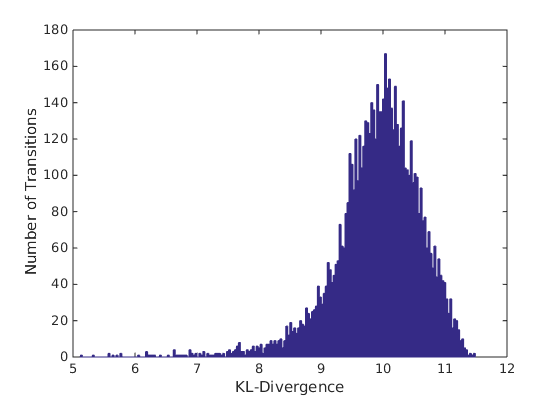
\includegraphics[width=0.45\textwidth]{images/divergence}
	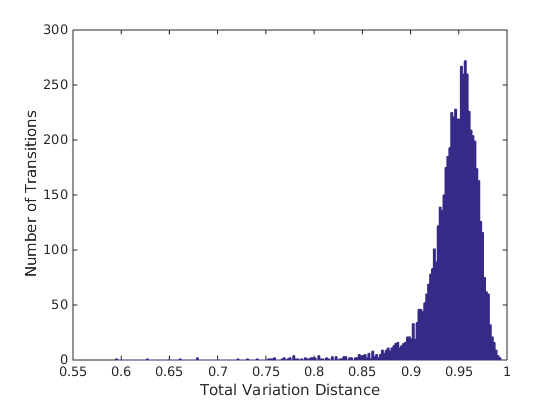
\includegraphics[width=0.45\textwidth]{images/totalvariation}
	\caption{Histogram of the value of the distance for Kullback-Leibler Divergence (left) and Total Variation (right)}
\end{center}
\end{figure}
As we can see, the distributions seem quite similar with a huge slope at some point: 8.5 for the KL-divergence and 0.9 for the total-variation distance. We found that we could choose either one or the other without a particular improvement as long as we set a sufficiently low threshold either way so as not to keep many meaningless transitions.

\subsection{Implementation}
\label{sec:EvoGraphImplementation}
\paragraph{}
The implementation of the evolution graph algorithm is quite straightforward. The algorithm receives an RDD of \emph{Theme} extracted by the EM algorithm that is repartitioned over a number of nodes usually equal to the number of \emph{time partitions}. The first step is to convert the objects \emph{Theme} into \emph{LightTheme} that contain only the information required by the computation of the distance in order to reduce memory usage and transfer times. The second step is to repartition the RDD of \emph{LightTheme} over a large enough number of executors in order for the cartesian product to be efficient. Finally, we apply a \emph{flatMap} over all the pairs to compute the distances and return or not the transitions. The hardest part of the algorithm is the computation of the divergence which requires a loop over all the words probability distributions and the computation of logarithms.


\subsection{Performance}
\label{sec:EvoGraphPerformance}
\paragraph{}
Even though we parallelize the work efficiently, the evolution graph algorithm does not fit the definition of scalable. Indeed, if we have twice as many periods of time and twice as many executors, then the running time does not stay the same. It will be in fact multiplied by two. This is due to the inherent quadratic complexity of the algorithm which requires to measure the distance for each pair of themes.

\paragraph{}
We could avoid this quadratic complexity by looking only at similarity between themes that are close to each other in time. For example, if we compute only transitions of less than one year for 200 years, the running time of the algorithm will be 200 times the running time for one year. However this simplification would make us lose interesting transitions for recurrent events like the Olympic Games happening every 4 years. 

\paragraph{}
We measured the performance of our algorithm over an increasing number of themes. For the test we used one week for the length of a time period and extracted 10 themes per week. This means 500 themes is approximately one year worth of themes.

\paragraph{}
\textbf{Measure of performance}\footnote{The execution time given is very inaccurate. The given values should only be taken as order of magnitude for the running time. The running time depends a lot on the time-span considered and the number of words in the extracted themes.}\textbf{ :}~\\
~\newline
\begin{tabular}{l|l|l|l}
\label{tab:quadratic}
Number of Theme & Number of pairs & Number of executors & Execution time \\ \hline
50 & 1250 & 500 & 5 s \\
100 & 5000 & 500 & 17 s \\
500 & 125000 & 500 & 510 s \\
\end{tabular}

\subsection{Results}
\label{sec:EvoGraphResults}

\paragraph{}
After computing all the Evolutionary Transitions, a graphical representation of the transition graph is generated using GraphViz. This is done by writing a .dot file from the Spark algorithm and the previously computed evolution graph RDD. This file is then easily interpreted to construct the desired graph for a given time-span. Figure \ref{fig:graph} shows a very small sub-graph generated by our algorithm. 

\begin{figure}[H]
\begin{center}
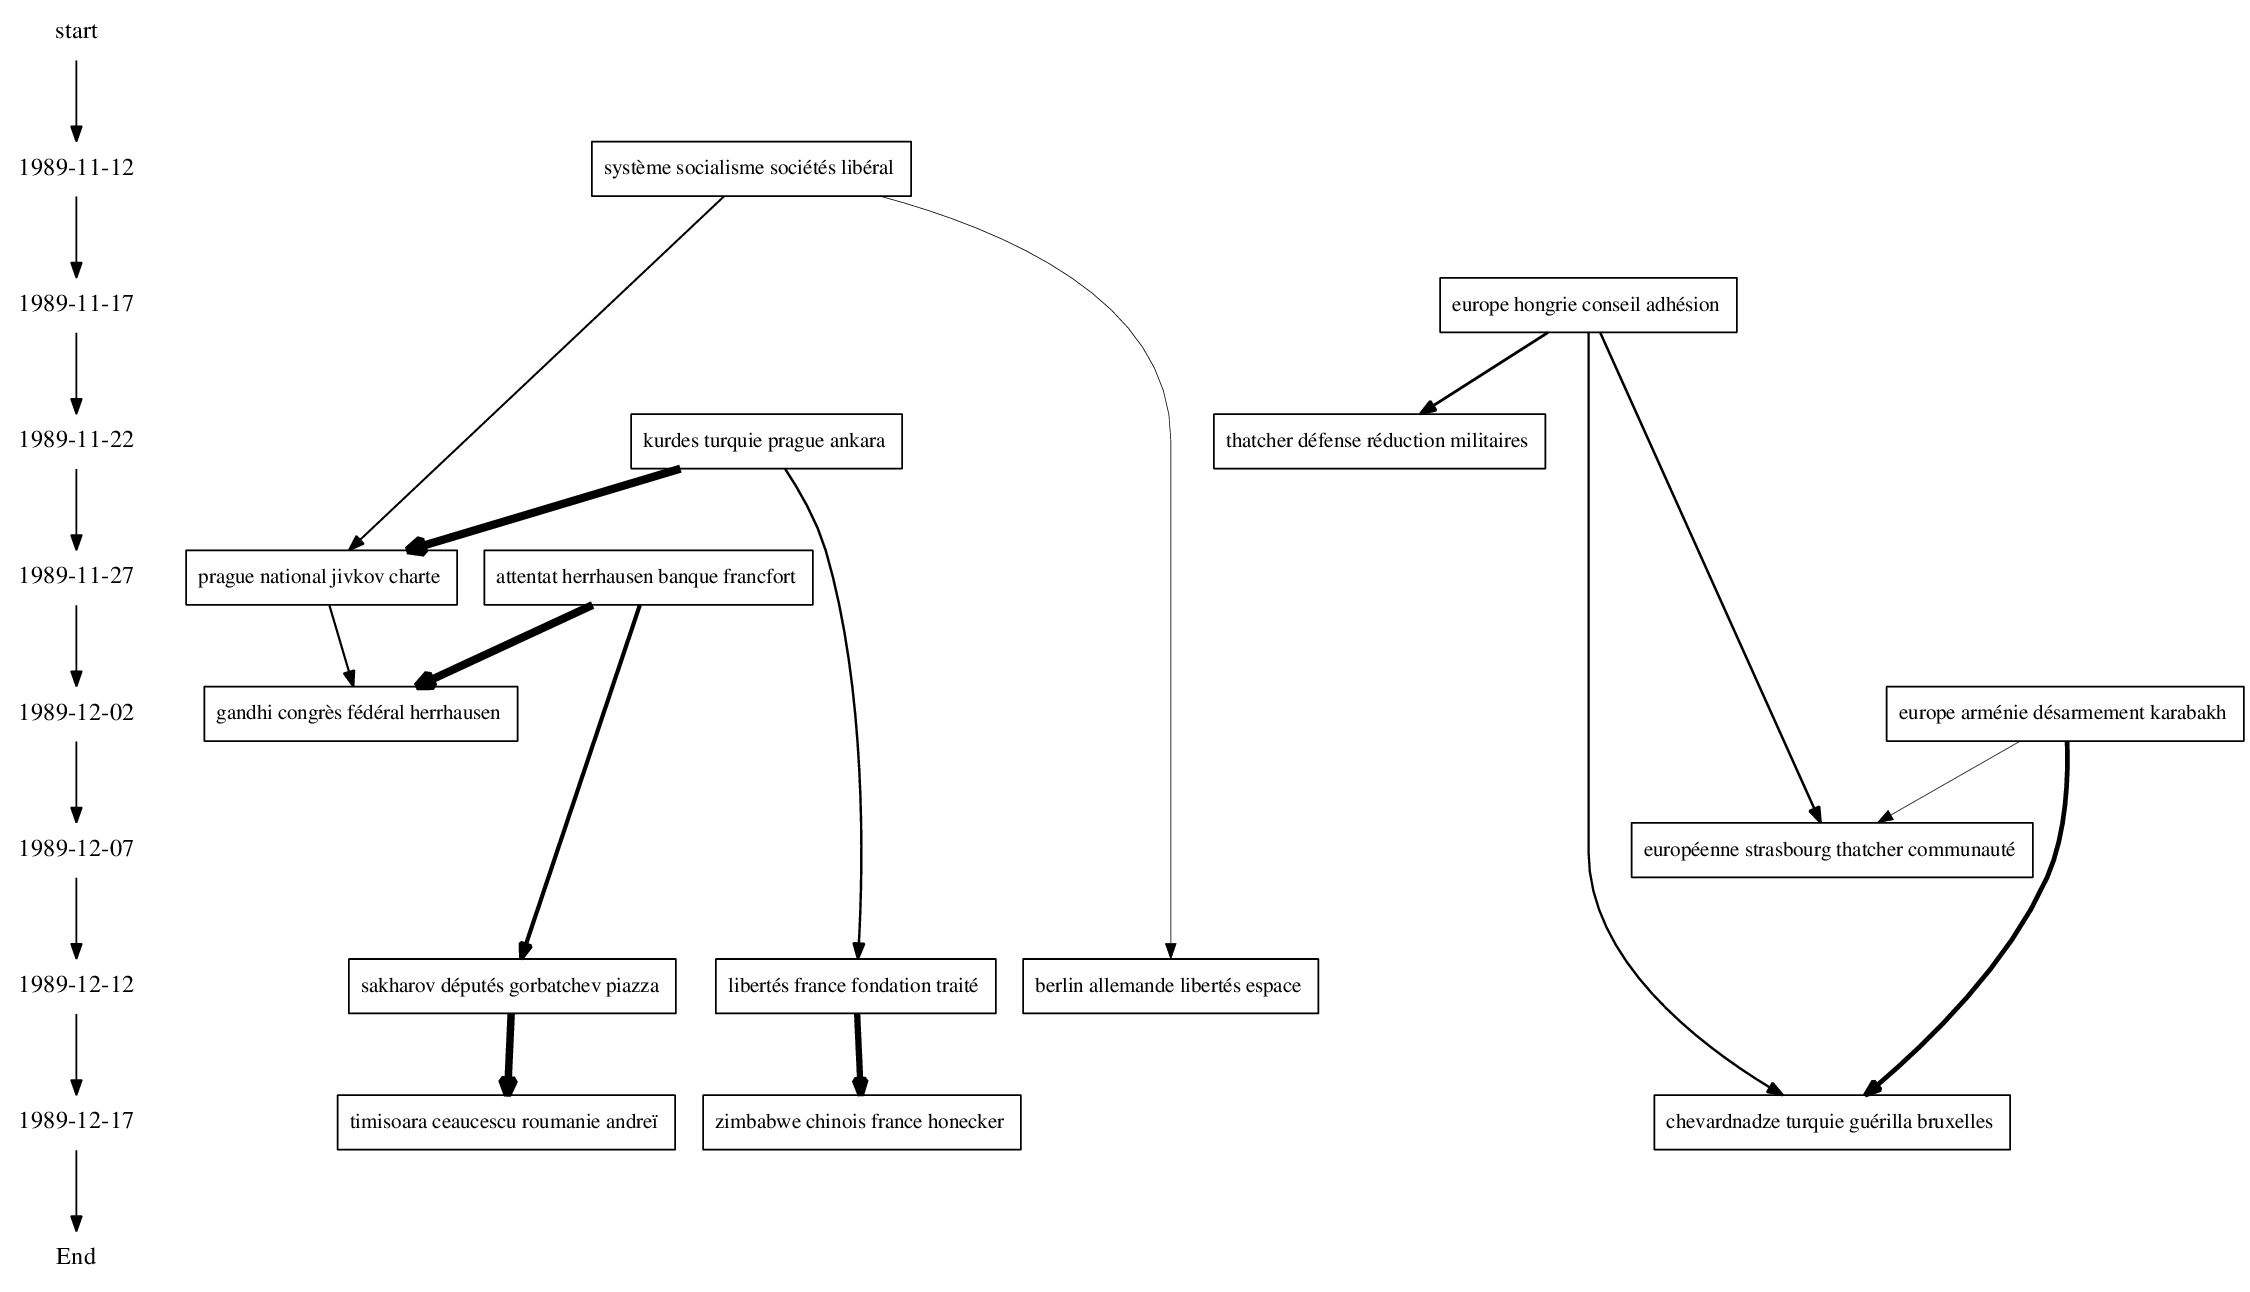
\includegraphics[width=0.9\textwidth]{images/graph.png}
\caption{Graph generated with GraphViz}
\label{fig:graph}
\end{center}
\end{figure}
